\documentclass[journal]{IEEEtran}

\usepackage[pdfpagemode={UseOutlines},bookmarks=true,bookmarksopen=true,
   bookmarksopenlevel=0,bookmarksnumbered=true,hypertexnames=false,
   colorlinks,linkcolor={blue},citecolor={blue},urlcolor={blue},
   pdfstartview={FitV},unicode,breaklinks=true]{hyperref}

% *** MATH PACKAGES ***
\usepackage{amsmath,amssymb,bm}

% *** GRAPHICS RELATED PACKAGES ***
\ifCLASSINFOpdf
	\usepackage[pdftex]{graphicx}
	\graphicspath{{images/}}
	% \DeclareGraphicsExtensions{.pdf,.jpeg,.png}
\else
	\usepackage[dvips]{graphicx}
	\graphicspath{{images/}}
	% \DeclareGraphicsExtensions{.eps}
\fi

% *** SUBFIGURE PACKAGES ***
\ifCLASSOPTIONcompsoc
  \usepackage[caption=false,font=normalsize,labelfont=sf,textfont=sf]{subfig}
\else
  \usepackage[caption=false,font=footnotesize]{subfig}
\fi

\usepackage[pdftex,dvipsnames]{xcolor}
\usepackage{listings,xargs}
\usepackage[colorinlistoftodos,prependcaption,textsize=tiny]{todonotes}

\definecolor{dkgreen}{rgb}{0,0.6,0}
\definecolor{gray}{rgb}{0.5,0.5,0.5}
\definecolor{mauve}{rgb}{0.58,0,0.82}
\newcommand{\fsize}{\scriptsize}
%\newcommand{\fsize}{\tiny}
\newcommand{\tabsize}{4}

\lstdefinelanguage{diff}{
  morecomment=[f][\color{blue}]{@@},		% group identifier
  morecomment=[f][\color{red}]-,		% deleted lines
  morecomment=[f][\color{dkgreen}]+,		% added lines
  morecomment=[f][\color{magenta}]{---},	% Diff header lines (must appear after +,-)
  morecomment=[f][\color{magenta}]{+++},
}

\lstset{frame=tb,
  language=C++,
%  aboveskip=0mm,
  belowskip=0mm,
  showstringspaces=false,
  columns=flexible,
  basicstyle={\fsize\ttfamily},
  numberstyle=\fsize\color{gray},
%  numbers=left,
  keywordstyle=\color{blue},
  commentstyle=\color{dkgreen},
  stringstyle=\color{mauve},
  breaklines=true,
  breakatwhitespace=true,
  tabsize=\tabsize
}

% correct bad hyphenation here
\hyphenation{op-tical net-works semi-conduc-tor}

\newcommand{\fref}[1]{\figurename~\ref{#1}}
\newcommand{\eref}[1]{(\ref{#1})}
\newcommand{\tref}[1]{\tablename~\ref{#1}}
\newcommand{\lref}[1]{LISTING~\ref{#1}}

\newcommandx{\improv}[2][1=]{\todo[linecolor=Plum,backgroundcolor=Plum!25,bordercolor=Plum,#1]{#2}}
\newcommand{\improvi}[1]{\improv[inline]{#1}}

\begin{document}

% paper title
\title{Acceleration of An SVM Classifier}

% author names and IEEE memberships
\author{Group 6: Yubo~Zhi (yz4116), Jiayang~Sun (js11815)}

% The paper headers
\markboth{ADSD Design Coursework}%
{ADSD Design Coursework}

% make the title area
\maketitle

\begin{abstract}
This course work aims to design and optimise a hardware Support Vector Machine (SVM) classifier on an embedded system using High Level Synthesis (HLS) language. The hardware implementation was optimised by various directives in HLS. In addition, the performance of software and hardware implementations were also assessed and compared in this excise.
\end{abstract}

\section{Introduction}

Dedicated hardware accelerators can perform a particular task faster then generalised software design. However, there are a few trade-offs associated with using hardware accelerators. In this exercise, an SVM classifier IP core was developed and optimised using Vivado HLS toolkit. The hardware platform used in this exercise is Zedboard, which include a Xilinx Zynq SoC FPGA. This FPGA has an ARM Cortex-A9 core together with the FPGA fabric. Hardware acceleration modules developed on the FPGA fabric can communicate with the ARM core through AXI interconnect. The procedure of designing and optimising the accelerator will be explained in details. Finally, the performance differences between hardware and software implementations were evaluated and discussed.

\hfill \today

\section{IP core implementation}

\subsection{Overview}

\fref{fig:ip} shows the purposed SVM classifier accelerator architecture, designed according to \eref{eq:cls}.

\begin{align}
	f(\bm{x}) &= sgn \left( bias + \sum_{i=1}^{N_{SV}} \alpha_i k(\bm{{sv}_i}, \bm{x}) \right)
	\label{eq:cls}\\
	\text{where}~k(\bm{x}, \bm{y}) &= 2 tanh(\bm{x} \cdot \bm{y})
\end{align}

\begin{figure}[ht]
	\centering
	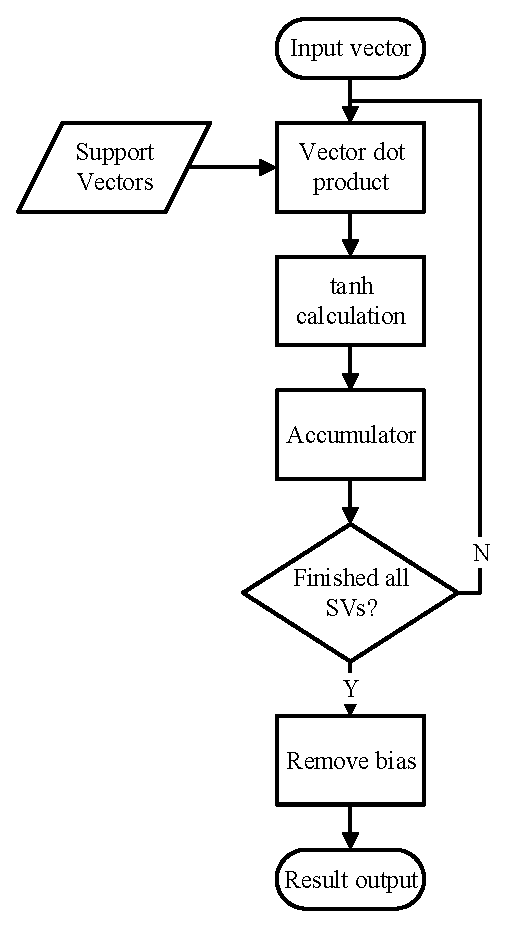
\includegraphics[width=0.6\columnwidth]{IP}
	\caption{Flow chart of purposed SVM classifier IP core}
	\label{fig:ip}
\end{figure}

According to the provided sample data, vectors have a width of 16 elements and there are 1050 support vectors. These numbers were replaced by macro definitions in the design, which can be easily adjusted to meet the properties of potentially other sample data.

\subsection{Dot product calculation}

Dot product between 2 vectors was calculated using the module designed previously in Part I.


\subsection{\texttt{tanh} calculation}

COordinate Rotation DIgital Computer (CORDIC) \cite{volder1959cordic} was used to calculate the \texttt{tanh} function.

\subsubsection{CORDIC}

CORDIC calculates trigonometric functions through vector rotation in 2-dimension space. It can be generalised to calculate \texttt{sinh} and \texttt{cosh} functions. The computations involved with CORDIC are simple integer addition, subtraction and shifting. This makes it suitable to use on a resource constrained embedded platform.

\subsubsection{Range and precision}\label{subsubsec:range}

The precision of CORDIC can be improved by allowing more iterations, however, the input range of CORDIC is non-ideal. The CORDIC implementation used in this design has an input range of about $\pm 1.10$ radians, but the sample dataset can give an input as large as $83.6$ radians.

In order to improve the performance of the \texttt{tanh()}, the algorithm for optimising range detection for CORDIC based on the trigonometric rules were implemented. 

\begin{align}
\sinh(\theta + \alpha) = \cosh(\theta)\sinh(\alpha) + \sinh(\theta)\cosh(\alpha)
\label{eq:tri}\\
\cosh(\theta + \alpha) = \cosh(\theta)\cosh(\alpha) + \sinh(\theta)\sinh(\alpha)
\end{align}

As equations \eref{eq:tri} describe, the $\theta$ can be used as a offset in order to increase the range of CORDIC.  In addition, declare a flag (\texttt{neg})to store whether the input is negative. If it is negative set the flag to one and invert the value to positive. Furthermore, it is easy to observe that $tanh()$ is infinitely approximate to 1 when the angle lager than 6 \texttt{rads}. As the result, when the input angle is larger than 6 \texttt{rads}, the result will be directly equal to \texttt{1}. Otherwise, the \texttt{trigo\_index} will be equal to the \texttt{round(theta)}. Also, \texttt{trigo\_index} is the index of look up table(LUT) of \texttt{lut\_sinh[]} and \texttt{lut\_cosh[]}. These value is used as the offset $\theta$ in the previous equation \eref{eq:tri}. After that the rest part of the result will be calculated inside \texttt{cordic()}. The results from \texttt{cordic()} can be used as $\alpha$ in equation \eref{eq:tri}. Moreover, do the operation from trigonometric rules inside \lref{lst:ext}, it will combine the results from CORDIC and offset in order to get the final output. Finally, if the \texttt{neg} is one, invert the output to negative. \cite{llamocca2007fixed}

\begin{lstlisting}[caption={Extending the range of CORDIC},captionpos=b,label=lst:ext]
	if (theta >= (mdata_t)6.0) {
		result = 1.0;
	} else {
		// Trigo index to extend range
		int trigo_index = theta;
		theta = theta - trigo_index;
		// Call Cordic function
		ldata_t outcosh, outsinh;
		cordic(theta, &outcosh, &outsinh);
		// Trigo rules
		result_sinh = (lut_sinh[trigo_index] * outcosh + lut_cosh[trigo_index] * outsinh);
		result_cosh = (lut_cosh[trigo_index] * outcosh + lut_sinh[trigo_index] * outsinh);
		result = result_sinh / result_cosh;
		*output = neg ? (ldata_t)-result : result;
	}
\end{lstlisting}

\subsection{SVM classifier}

The top-level SVM classifier was designed according to the flow chart \fref{fig:ip}. It iterates through all support vectors, accumulates each result, finally output a boolean value according to the sign of accumulator after bias removal. The function \texttt{k()} is the same as the k inside of equation \eref{eq:cls}. It will calculate the dot product of two vectors, and apply \texttt{tanh()} to the dot product in order to get the output. Finally, output will be checked whether it is negative. If it is positive, then output 0, otherwise output 1.

\begin{lstlisting}[caption={Top-level SVM classifier},captionpos=b,label=lst:clas]
static void k(ldata_t u[N], ldata_t v[N], ldata_t *output)
{
	mdata_t res;
	dotp(u, v, &res);
	res = res << 1u;	// * 2
	fp_tanh(res, output);
}

void classifier(ldata_t x[N], int *output)
{
	hdata_t sum = 0;
	for (int i = 0; i != ASIZE(alpha); i++) {
		ldata_t res;
		k(SVs[i], x, &res);
		sum += res * alpha[i];
	}
	*output = sum + bias >= 0 ? 0 : 1;
}	
\end{lstlisting}

\subsection{Hardware verification}

\subsubsection{Test bench}

The design of SVM classifier was verified using C simulation test benches. The test bench iterates through all \texttt{testData} vectors from the sample dataset and executes the classifier. The results from classifier were compared with \texttt{testDataLabel} ground truths from the same sample dataset. Any difference will be recorded, and an overall error rate will be calculated at the end of simulation.

\subsubsection{Reference generation}

A double precision example classifier implementation was available from the dataset. It produces 170 incorrect results from all 2000 ground truths values, corresponding to an error rate of $8.5 \%$. The results including errors from the double precision were considered the reference output, therefore it can reflect any precision mismatches between the hardware implementation and software double precision implementation.

\subsection{Design evaluation}

The original implementation without any optimisation directives gives a maximum latency of 164877 clock cycles, as shown by \tref{tbl:res_unopt}.

\begin{table}[ht]
	% increase table row spacing, adjust to taste
	\renewcommand{\arraystretch}{1.3}
	\caption{Performance and resource usage of unoptimised version}
	\label{tbl:res_unopt}
	\centering
	% Some packages, such as MDW tools, offer better commands for making tables
	% than the plain LaTeX2e tabular which is used here.
	\begin{tabular}{llll}
		\hline
		Item			& Unoptimised	\\
		\hline
		Estimated clock timing	& $8.77$	\\
		Latency			& $164877$	\\
		Interval		& $164878$	\\
		Co-simulation (average)	& $203$		\\
		\hline
		BRAM\_18K		& $36~(12\%)$	\\
		DSP48E			& $6~(2\%)$	\\
		FF			& $1436~(1\%)$	\\
		LUT			& $4086~(7\%)$	\\
		\hline
	\end{tabular}
\end{table}

Running RTL co-simulation using all 2000 test vectors with this order of delay interval between every test vector will be very time-consuming and not very useful. Therefore, only C simulation was used to ensure the correctness of the unoptimised design. RTL co-simulations were still used in later optimised design.

\section{Performance optimisation}

\subsection{Interface optimisation}

The interface for specified input vectors was optimised by reducing the interface width to a minimum and using the \texttt{ARRAY\_RESHAPE} directive. This directive can combine multiple elements of the input vector to a single 32-bit buffer, reduces the number of data transfers needed between the ARM core and the hardware accelerator.

\subsection{Throughput optimisation}

\subsubsection{Pipelining}

By using the technique of pipelining, the throughput can be greatly improved without significant increases of hardware resource usages. This can be achieved by applying the \texttt{PIPELINE} directive. Vivado HLS will automatically insert pipeline stage registers in appropriate locations. An iteration interval of 1 clock cycles was achieved by pipelining. With the addition of a few pipeline stages filling the entire pipeline beforehand, the iteration of all 1050 support vectors now takes only over 1100 clock cycles.

\subsubsection{Loop unrolling}

There are also some small iteration loops in the design, such as the iteration inside dot product calculation which only iterates about 16 times. These loops can be unrolled to allow parallel computation of iterations, at the cost of more hardware resource usages. This can be achieved by applying the \texttt{UNROLL} directive. Vivado HLS is capable of duplicating the loop body multiple times, and applying map-reduce techniques to resolve dependencies automatically. Together with pipelining, this can reduce the number of pipeline stages.

\subsubsection{Parallel chains}

The latency can be further reduced by executing multiple iterations of the support vector loop inside the main classifier function in parallel. Instead of sequentially iterates through all 1050 support vectors, ideally this parallel execution can reduce the latency by a factor of parallel chains.
The disadvantage of this method is, the hardware resource usage will be increased by the same factor in order to implement multiple parallel chains. A trade-off between throughput and resource usage is implied.
This parallel execution was done by unrolling the main loop while specifying unroll factor. All constant values such as support vectors and alpha implemented by ROMs need to be partitioned by the same factor to prevent Vivado duplicating the entire ROM for each parallel chain. The array partition was done by specifying the \texttt{ARRAY\_PARTITION} directive.

\improvi{Insert codes?}

\subsection{Clock timing issue}

An unexpected issue occurred when applying unroll optimisations. The target clock period specified for this design is $10 ns$, but Vivado kept generating paths exceeding that clock constrain. By analysing the warning messages about the critical path, it is possible to resolve this issue by separating the arithmetic involved in the critical path, letting Vivado insert pipeline registers between them.

An example of resolving the timing issue is given by \lref{lst:tim}. The original multiplication and accumulation operation was broken into 10 separate \texttt{sums} variables as caches, partitioned to match the loop unroll factor. So that each parallel chain has a dedicated accumulator, summarised together in later stages. This removes the need for accumulate all 10 parallel chains in each iteration, hence reduces the length of the critical path.

\begin{lstlisting}[language=diff,caption={Code modification to resolve timing issue},captionpos=b,label=lst:tim]
--- old/classifier.cpp
+++ new/classifier.cpp
@@ -62,12 +62,19 @@ void classifier(ldata_t x[N],
 #pragma HLS INTERFACE s_axilite port=output
 #pragma HLS INTERFACE s_axilite port=return
     hdata_t sum = 0;
+    hdata_t sums[10] = {0, 0, 0, 0, 0, 0, 0, 0, 0, 0};
+#pragma HLS ARRAY_PARTITION variable=sums cyclic factor=10 dim=1
     for (int i = 0; i != ASIZE(alpha); i++) {
 #pragma HLS PIPELINE
 #pragma HLS UNROLL factor=10
        ldata_t res;
        k(SVs[i], x, &res);
-       sum += res * alpha[i];
+       sums[i % 10] += res * alpha[i];
+    }
+    for (int i = 0; i != 10; i++) {
+#pragma HLS PIPELINE
+#pragma HLS UNROLL
+       sum += sums[i];
     }
     *output = sum + bias >= 0 ? 0 : 1;
 }
\end{lstlisting}

\subsection{New \texttt{tanh()} reflection}
As the subsection \ref{subsubsec:range} mentioned, there is a new technique to enhance the range and accuracy of the \texttt{tanh()} fuction. However, it needs more resource and more instructions to complete, which means that it has higher latency than the previous CORDIC (133 cycles). However, the final latency of the design is shown in \fref{latency}, which is 150 cycle. Although there are 17 more cycles to complete the calculation, it gets as accurate as the double precision answer generated by software test bench. Because if using the previous method to complete \texttt{tanh()} there are in total 169 errors, nonetheless it is different from the result come from the test bench which is 170 errors. As the result, the final implementation choose a more accuracy method in order to get enhanced classification.   

\subsection{Design verification}

Correctness verifications by C simulations were done after every optimisations and code modifications, using the golden reference output generated from double precision implementation.

An unexpected discrepancy between Vivado HLS' C language and ISO C language standard (6.7.8.19 \cite{iso1999iec}) was discovered. All array elements must be explicitly initialised in Vivado HLS for a defined behaviour, whereas in ISO C standard, uninitialised elements in a partially initialised array should have the value 0, the same as static storage initialisation. Hence the 10 zeros written in the initialisation of \texttt{sums} in \lref{lst:tim}.

After applied all optimisations, the latency reduced significantly. RTL co-simulation was done at this stage before exporting as an IP core, to ensure the exported RTL implementation has the same functionality as the C implementation.

\subsection{Design evaluation}

\fref{fig:latency} shows the latency and varies aspects of hardware resources versus main loop unrolling factor.

\begin{figure}[ht]
	\centering
	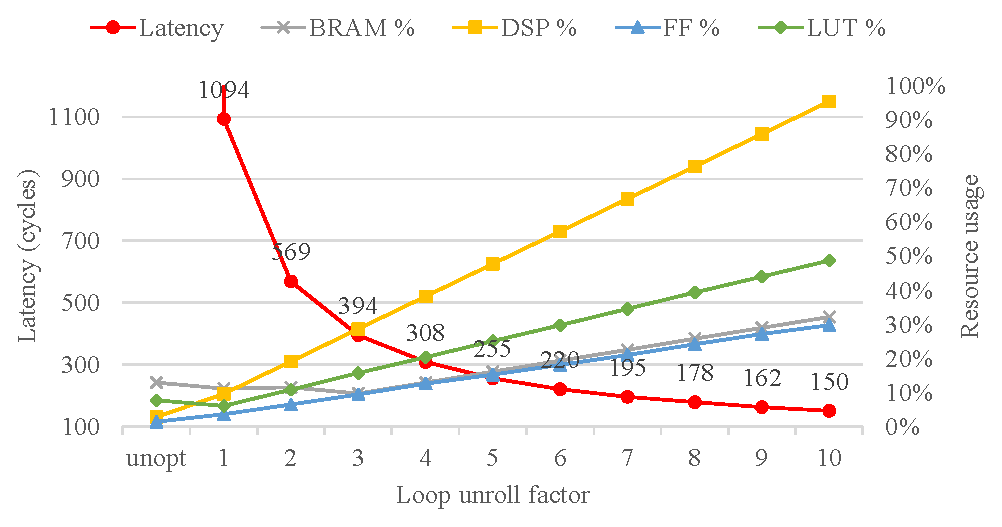
\includegraphics[width=\columnwidth]{latency}
	\caption{Latency and resource usage versus loop unrolling}
	\label{fig:latency}
\end{figure}

As loop unroll factor increases, hardware resource usages increase linearly. However, the effect on latency decreases exponentially. The latency can be estimated by \eref{eq:latency}.

\begin{equation}
	\text{latency} = \frac{N_{SV}}{\text{factor}} + \text{stages}
	\label{eq:latency}
\end{equation}

$N_{SV}$ equals the number of support vectors, which is 1050. Stages is the depth of pipeline, which is 44 in most cases, given by the loop latency value.

The equation shows, there is always some factors that can not be parallelised. Therefore the effect on performance will become more and more insignificant. Moreover, with a loop unroll factor of 10, DSP resource usage had already reached $95.45 \%$, impossible for further adjustments.

\improvi{More?}

\section{System implementation}

After multiple optimisations, the improved implementation was packaged into Vivado as an IP core. The setup of Vivado and SDK were the same as in previous dot product exercise. \fref{fig:sdk} describes an abstract structural overview of the testing program running on the ARM core, developed on the SDK.

\begin{figure}[t]
	\centering
	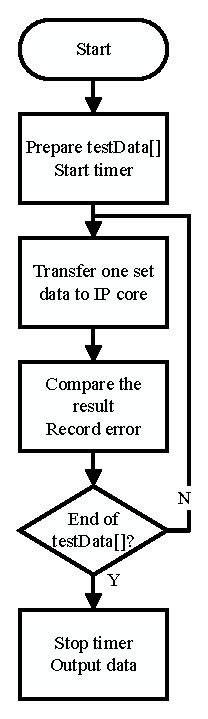
\includegraphics[width=0.3\columnwidth]{sdk}
	\caption{Overview of the testing program}
	\label{fig:sdk}
\end{figure}

\section{System evaluation}

\subsection{Performance and resource usage}

Using the global timer inside ARM core, it is possible to get cycle accurate profiling information.

The support vector classifier was also implemented as software using double precision and fixed point CORDIC inside the ARM core, as a performance comparison to hardware implementation.

The performance data of software and notable hardware implementations are summarised in \tref{tbl:throughput}. \fref{fig:throughput} shows detailed hardware implementation throughputs and resource usage values. Both polling and interrupt methods for waiting results ready were implemented, however, only performance data from polling method was shown. The polling method gives slightly better overall performance values, probably due to some interfacing overheads of supporting interrupt.

\begin{table}[ht]
	% increase table row spacing, adjust to taste
	\renewcommand{\arraystretch}{1.3}
	\caption{Performance and resource usages of system implementations}
	\label{tbl:throughput}
	\centering
	% Some packages, such as MDW tools, offer better commands for making tables
	% than the plain LaTeX2e tabular which is used here.
	\begin{tabular}{llll}
		\hline
		Type			& Throughput (k vectors / second)	\\
		\hline
		Double precision	& $2.96$	\\
		Fixed precision CORDIC	& $6.64$	\\
		\hline
		Unoptimised hardware	& $1.47$	\\
		Pipelined hardware	& $152.17$	\\
		Unrolled with factor 10	& $541.18$	\\
		\hline
	\end{tabular}
\end{table}

\begin{figure}[t]
	\centering
	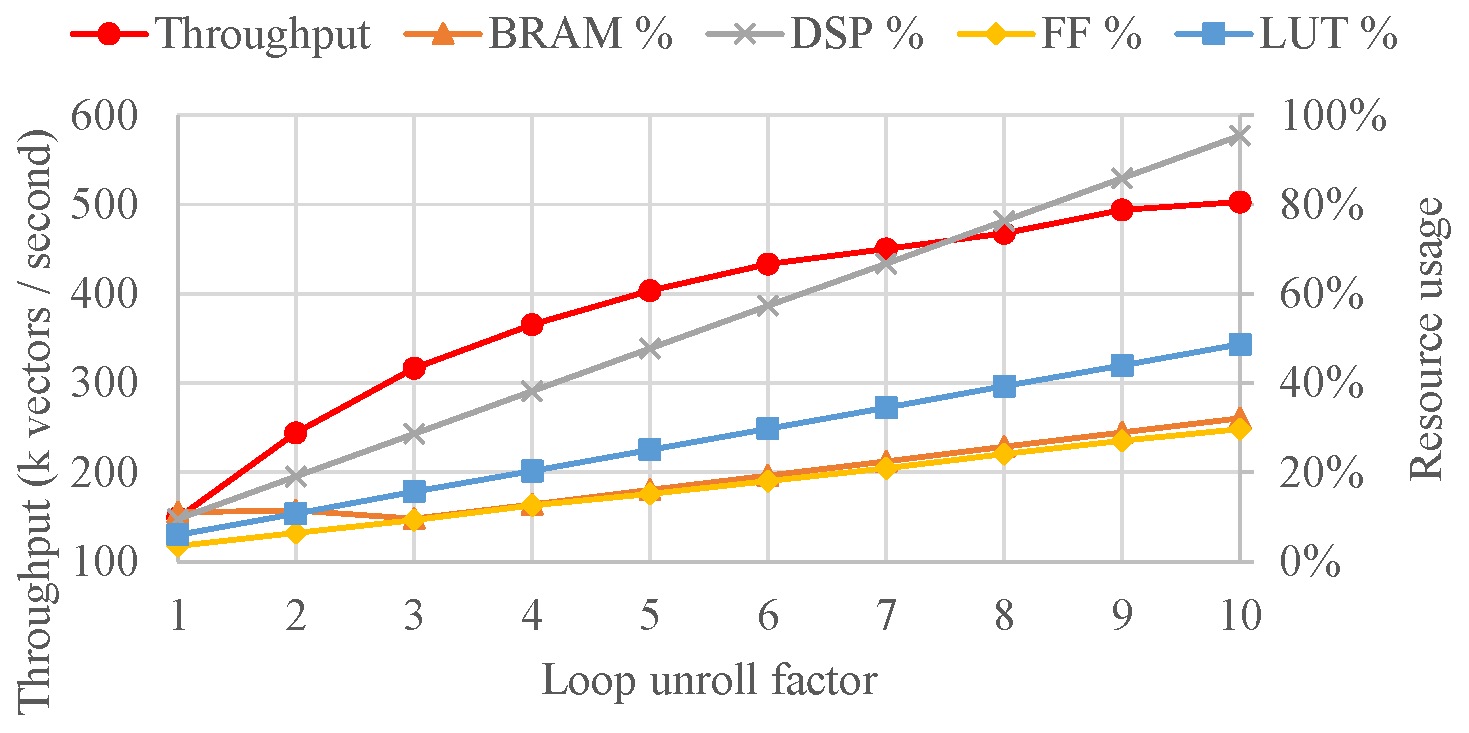
\includegraphics[width=\columnwidth]{throughput}
	\caption{System throughput and resource usages versus loop unroll factor}
	\label{fig:throughput}
\end{figure}

\subsection{Reflection and Limitations}

\section{Conclusion}

By evaluating the performance data of software and hardware implementation of the same algorithm, the advantages, use case and limiting factors of using hardware accelerators were investigated. Although the computation speed of dedicated hardware accelerator can be faster than software implementation, the data transfer performance may limit the actual efficiency.

% References section
\bibliographystyle{IEEEtran}
\bibliography{Reference}

% that's all folks
\end{document}
